% ============================================================================
% Droites concourantes : les trois medianes du triangle
% Extrait de la fiche : Barycentres et lignes de niveau (classe de 1ere D)
% Necessite \usepackage{tikz} et \usetikzlibrary{calc} (charges par le fichier principal)
% ============================================================================
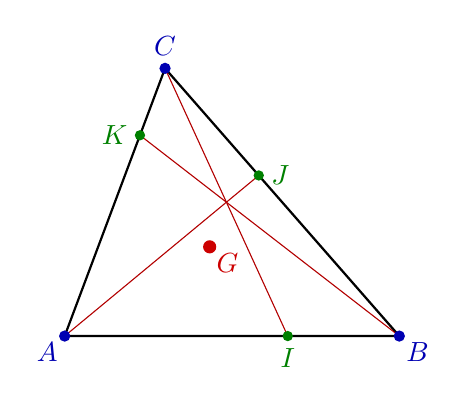
\begin{tikzpicture}[scale=0.85,>=latex]
  \coordinate (A) at (0,0); \coordinate (B) at (5,0); \coordinate (C) at (1.5,4);
  \coordinate (I) at (3.3333,0); \coordinate (J) at (2.9,2.4); \coordinate (K) at (1.125,3);
  \coordinate (G) at (2.1667,1.3333);
  \draw[thick] (A) -- (B) -- (C) -- cycle;
  \draw[thin,red!70!black] (C) -- (I);
  \draw[thin,red!70!black] (A) -- (J);
  \draw[thin,red!70!black] (B) -- (K);
  \fill[blue!70!black] (A) circle (2.4pt) node[below left=-1pt] {$A$};
  \fill[blue!70!black] (B) circle (2.4pt) node[below right=-1pt] {$B$};
  \fill[blue!70!black] (C) circle (2.4pt) node[above=1pt] {$C$};
  \fill[green!50!black] (I) circle (2.2pt) node[below=1pt] {$I$};
  \fill[green!50!black] (J) circle (2.2pt) node[right=1pt] {$J$};
  \fill[green!50!black] (K) circle (2.2pt) node[left=1pt] {$K$};
  \fill[red!80!black] (G) circle (2.8pt) node[below right=-1pt] {$G$};
\end{tikzpicture}
